\documentclass[10pt]{article}
\usepackage[utf8x]{inputenc}
\usepackage{polski}

\usepackage{amsmath}
\usepackage{amsthm}
\usepackage{amssymb}

\usepackage{graphics}
\usepackage{pdfpages}
\DeclareGraphicsRule{.1}{mps}{*}{}
\usepackage{epstopdf}

% \newcommand{\hint}[2]{\begin{flushleft}\textbf{\ref{#1}}\quad #2\end{flushleft}}

\usepackage{geometry}
\geometry{a4paper, margin=2cm}

\begin{document}
    
%NAGLOWEK

    \noindent
    \begin{minipage}{0.5\textwidth}
        \LARGE{\textsf{\textbf{Zadanie: WIE\\Wieżowce}}}
    \end{minipage}
    \begin{minipage}{0.5\textwidth}
        \begin{flushright}
            
\includegraphics[height=1.5cm]{logo.png}
        \end{flushright}
    \end{minipage}
    
    \noindent\rule{\textwidth}{0.4pt}
    
    \noindent\textbf{Akademia Programowania PWSW, dzień ?, Dostępna pamięć: 128 MB.}
    \vspace{1em}
    
%TRESC
    
    \noindent
    Bajtuś uwielbia bawić się klockami, a ostatnio fascynuje się również wielkimi metropoliami, których panoramy potrafi rysować z pamięci. Tym razem Bajtuś postanowił zbudować swoją metropolię przy pomocy jednostkowych sześciennych klocków. Chce aby miasto zostało wzniesione na planie prostokąta $n\times m$, którego zachodnią panoramę (długości $n$) i południową panoramę (długości $m$) zaprojektuje samodzielnie. Każda z narysowanych panoram określa jaką wysokość będzie miał najwyższy spośród stojących w danym rzędzie budynków. Bajtuś chciałby również, aby jego model (zbudowany z klocków na podstawie stworzonych panoram) ładnie się prezentował, zatem aby każdy ze zbudowanych wieżowców był jak najwyższy (zgodnie z narysowanymi panoramami) oraz aby wszystkie budynki w wybranych rzędach były zbudowane tylko z białych klocków. Budynki nienależące do wskazanych rzędów zostaną wybudowane z klocków w innych kolorach.
    
    Bajtuś zaprojektował już obie panoramy i dla każdego rzędu stwierdził czy wszystkie budynki powinny być białe, a teraz zastanawia się czy ma wystarczająco dużo białych klocków. Napisz program, który pomoże Bajtusiowi określić ile białych klocków potrzebuje, aby zbudować swoją metropolię.

%WEJSCIE

    \section*{Wejście}
    
    W pierwszym wierszu standardowego wejścia znajdują się dwie liczby całkowite $n$ i $m$ $(1 \leq n, m \leq 100000)$, oznaczające odpowiednio długość panoramy od strony zachodniej i od strony południowej. W $n$ kolejnych wierszach znajdują się dwie liczby całkowite $h_{i}$ $(1\leq h_{i}\leq 10^{6})$, oznaczającą wysokość najwyższego z budynków w danym rzędzie patrząc od strony zachodniej, i $c_{i}$ równą 1 jeżeli cały ten rząd powinien być zbudowany z białych klocków lub 0 w przeciwnym razie. W $m$ kolejnych wierszach znajdują się dwie liczby całkowite $h_{j}$ $(1\leq h_{j}\leq 10^{6})$, oznaczającą wysokość najwyższego z budynków w danym rzędzie patrząc od strony południowej, i $c_{j}$ równą 1 jeżeli cały ten rząd powinien być zbudowany z białych klocków lub 0 w przeciwnym razie.

%WYJSCIE

    \section*{Wyjście}
    
    Na standardowe wyjście należy wypisać jedną liczbę całkowitą, oznaczającą liczbę białych klocków które Bajtuś potrzebuje do zbudowania swojego modelu. Jeżeli Bajtuś pomylił się tworząc panoramy i model jest niemożliwy do zbudowania należy wypisać $-1$.

%PRZYKLAD

    \section*{Przykład}
    
    \noindent
    \begin{minipage}[t]{0.5\textwidth}
        Dla danych wejściowych:\vspace{1ex}\\
        \texttt{3 3\\3 1\\2 0\\1 0\\1 0\\2 1\\3 0}
    \end{minipage}
    \begin{minipage}[t]{0.5\textwidth}
        poprawnym wynikiem jest:\vspace{1ex}\\
        \texttt{9}
    \end{minipage}
    
    \vspace{-5em}
    \begin{center}
        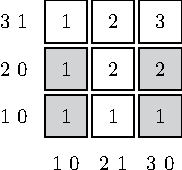
\includegraphics{wierys-1.pdf}
    \end{center}
    
%OCENIANIE

    \section*{Ocenianie}
        
    Zestaw testów dzieli się na następujące podzadania. Testy do każdego podzadania składają się z jednej lub większej liczby osobnych grup testów.
    
    \begin{center}
        \begin{tabular}{ |c|p{9cm}|c| }
            \hline
            \textbf{Podzadanie} & \textbf{Warunki} & \textbf{Liczba punktów}\\
            \hline
            1 & $1 \leq n, m \leq 1000$ & 30\\
            \hline
            2 & $c_{j} = 0$, dla wszytkich rzędów południowej panoramy & 30\\
            \hline
            3 & brak dodatkowych ograniczeń & 40\\
            \hline
        \end{tabular}
    \end{center}

\end{document}
\documentclass[10pt]{article}
\usepackage[utf8x]{inputenc}
\usepackage{polski}

